\section{3D Printing Toolchain}

\subsection{Extruder}

\indent

The extruder is the mechanism responsible for depositing the filament in a 3D printing system. Generally, this mechanism includes a motor that drives a gripping mechanism, which reels in and pushes the filament into a heated nozzle. The nozzle heats the filament into a \emph{mushy} state and lays the filament on the printing bed or on an already printed layer to create the part.\\

In the case of our carbon fiber 3D printer, the extruder is required to mount to the robot arm, be compact\footnote{The compact size is required for two reasons. First, to ensure that induced torque on the robot arm joints and gripper remain within safe operating conditions. Second, to readily permit the nozzle to deposit material when not perpendicular to the build platform, which will be required for printing curved layers.}, and accept filaments of a variety of sizes (likely ranging in diameter from 1.75 mm to 3 mm). Consideration was also placed on whether or not the gripper fixturing should accept FANUC and Puma mounting hardware and associated configurations, and if the extruder should also house the control electronics. By the time that these features were to be implemented in the design of the extruder, we had officially obtained access to the Fanuc robot. Subsequently, the extruder only needed to mount to the FANUC and did not need to secure the electronics board since wire management within the FANUC cage could be easily implemented.\\

Figure~\ref{fig:old extruder} presents the initial design of the extruder in \emph{SolidWorks}. The extruder mounts to the Fanuc grippers and is constructed out of a combination of machined aluminum parts and RepRap hardware (nozzle, J-head, J-head mounting plate, ceramic heating element, thermistor, fan, and fan mount). This configuration locates the nozzle outlet along the mid-plane of the grippers for simple coordinate transformations when programming the robot to print. Laser-cut acrylic gears provide a three-to-one step up in torque from the stepper motor and drive a notched screw, which grips and pushes the filament into the nozzle. A bearing opposite the screw provides counter-pressure and its mounting plates can adjust the distance between the screw and bearing to accommodate different filament sizes.\\

\begin{figure}[h!]
\centering
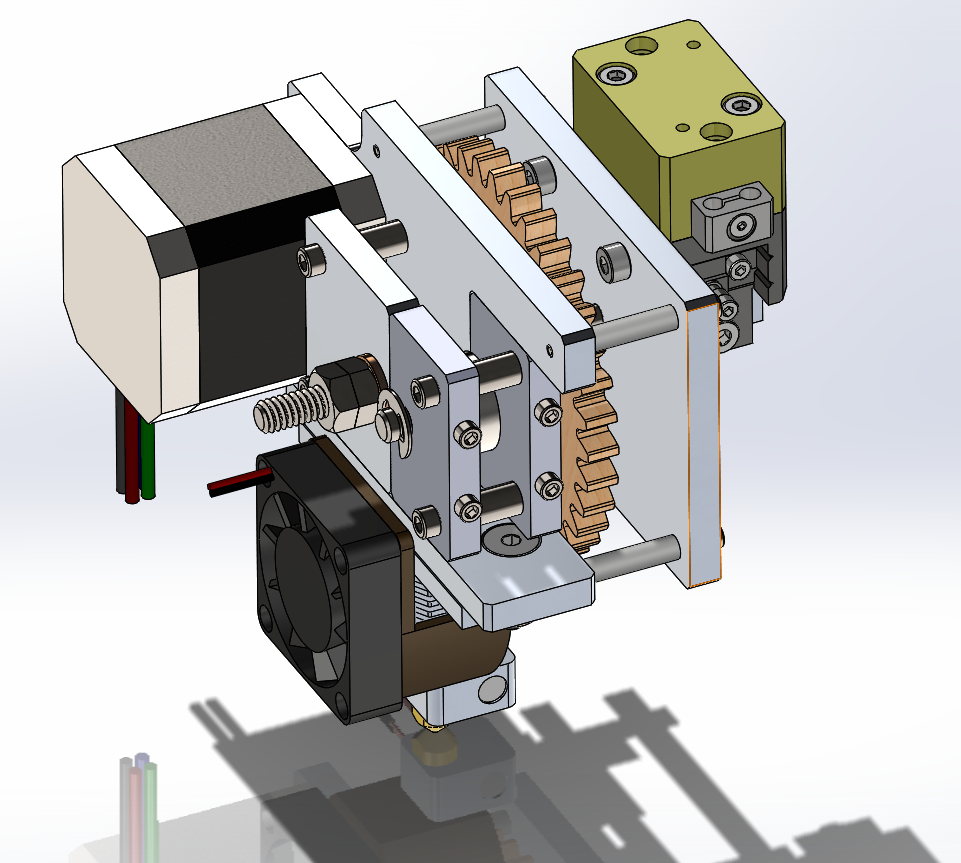
\includegraphics[width=0.5\textwidth]{./figures/extruder-old-2}
\caption{An isometric view of the initial extruder design.}
\label{fig:old extruder}
\end{figure}

To assess the feasibility of the initial extruder design, minor tweaks were implemented within the CAD to make a laser-cut prototype.  Figure~\ref{fig:prototype extruder} shows the prototype mounted on the FANUC grippers. The prototype served its purpose and demonstrated numerous problems with the initial design. There were some mis-measurements of RepRap hardware, using spacers instead of threaded standoffs decreased the rigidity of the structure, the structure was a bit larger than desired, and a few undetected interferences were discovered. Subsequently, the extruder then went through a series of redesigns to develop an acceptable configuration.\\

\begin{figure}[h!]
\centering
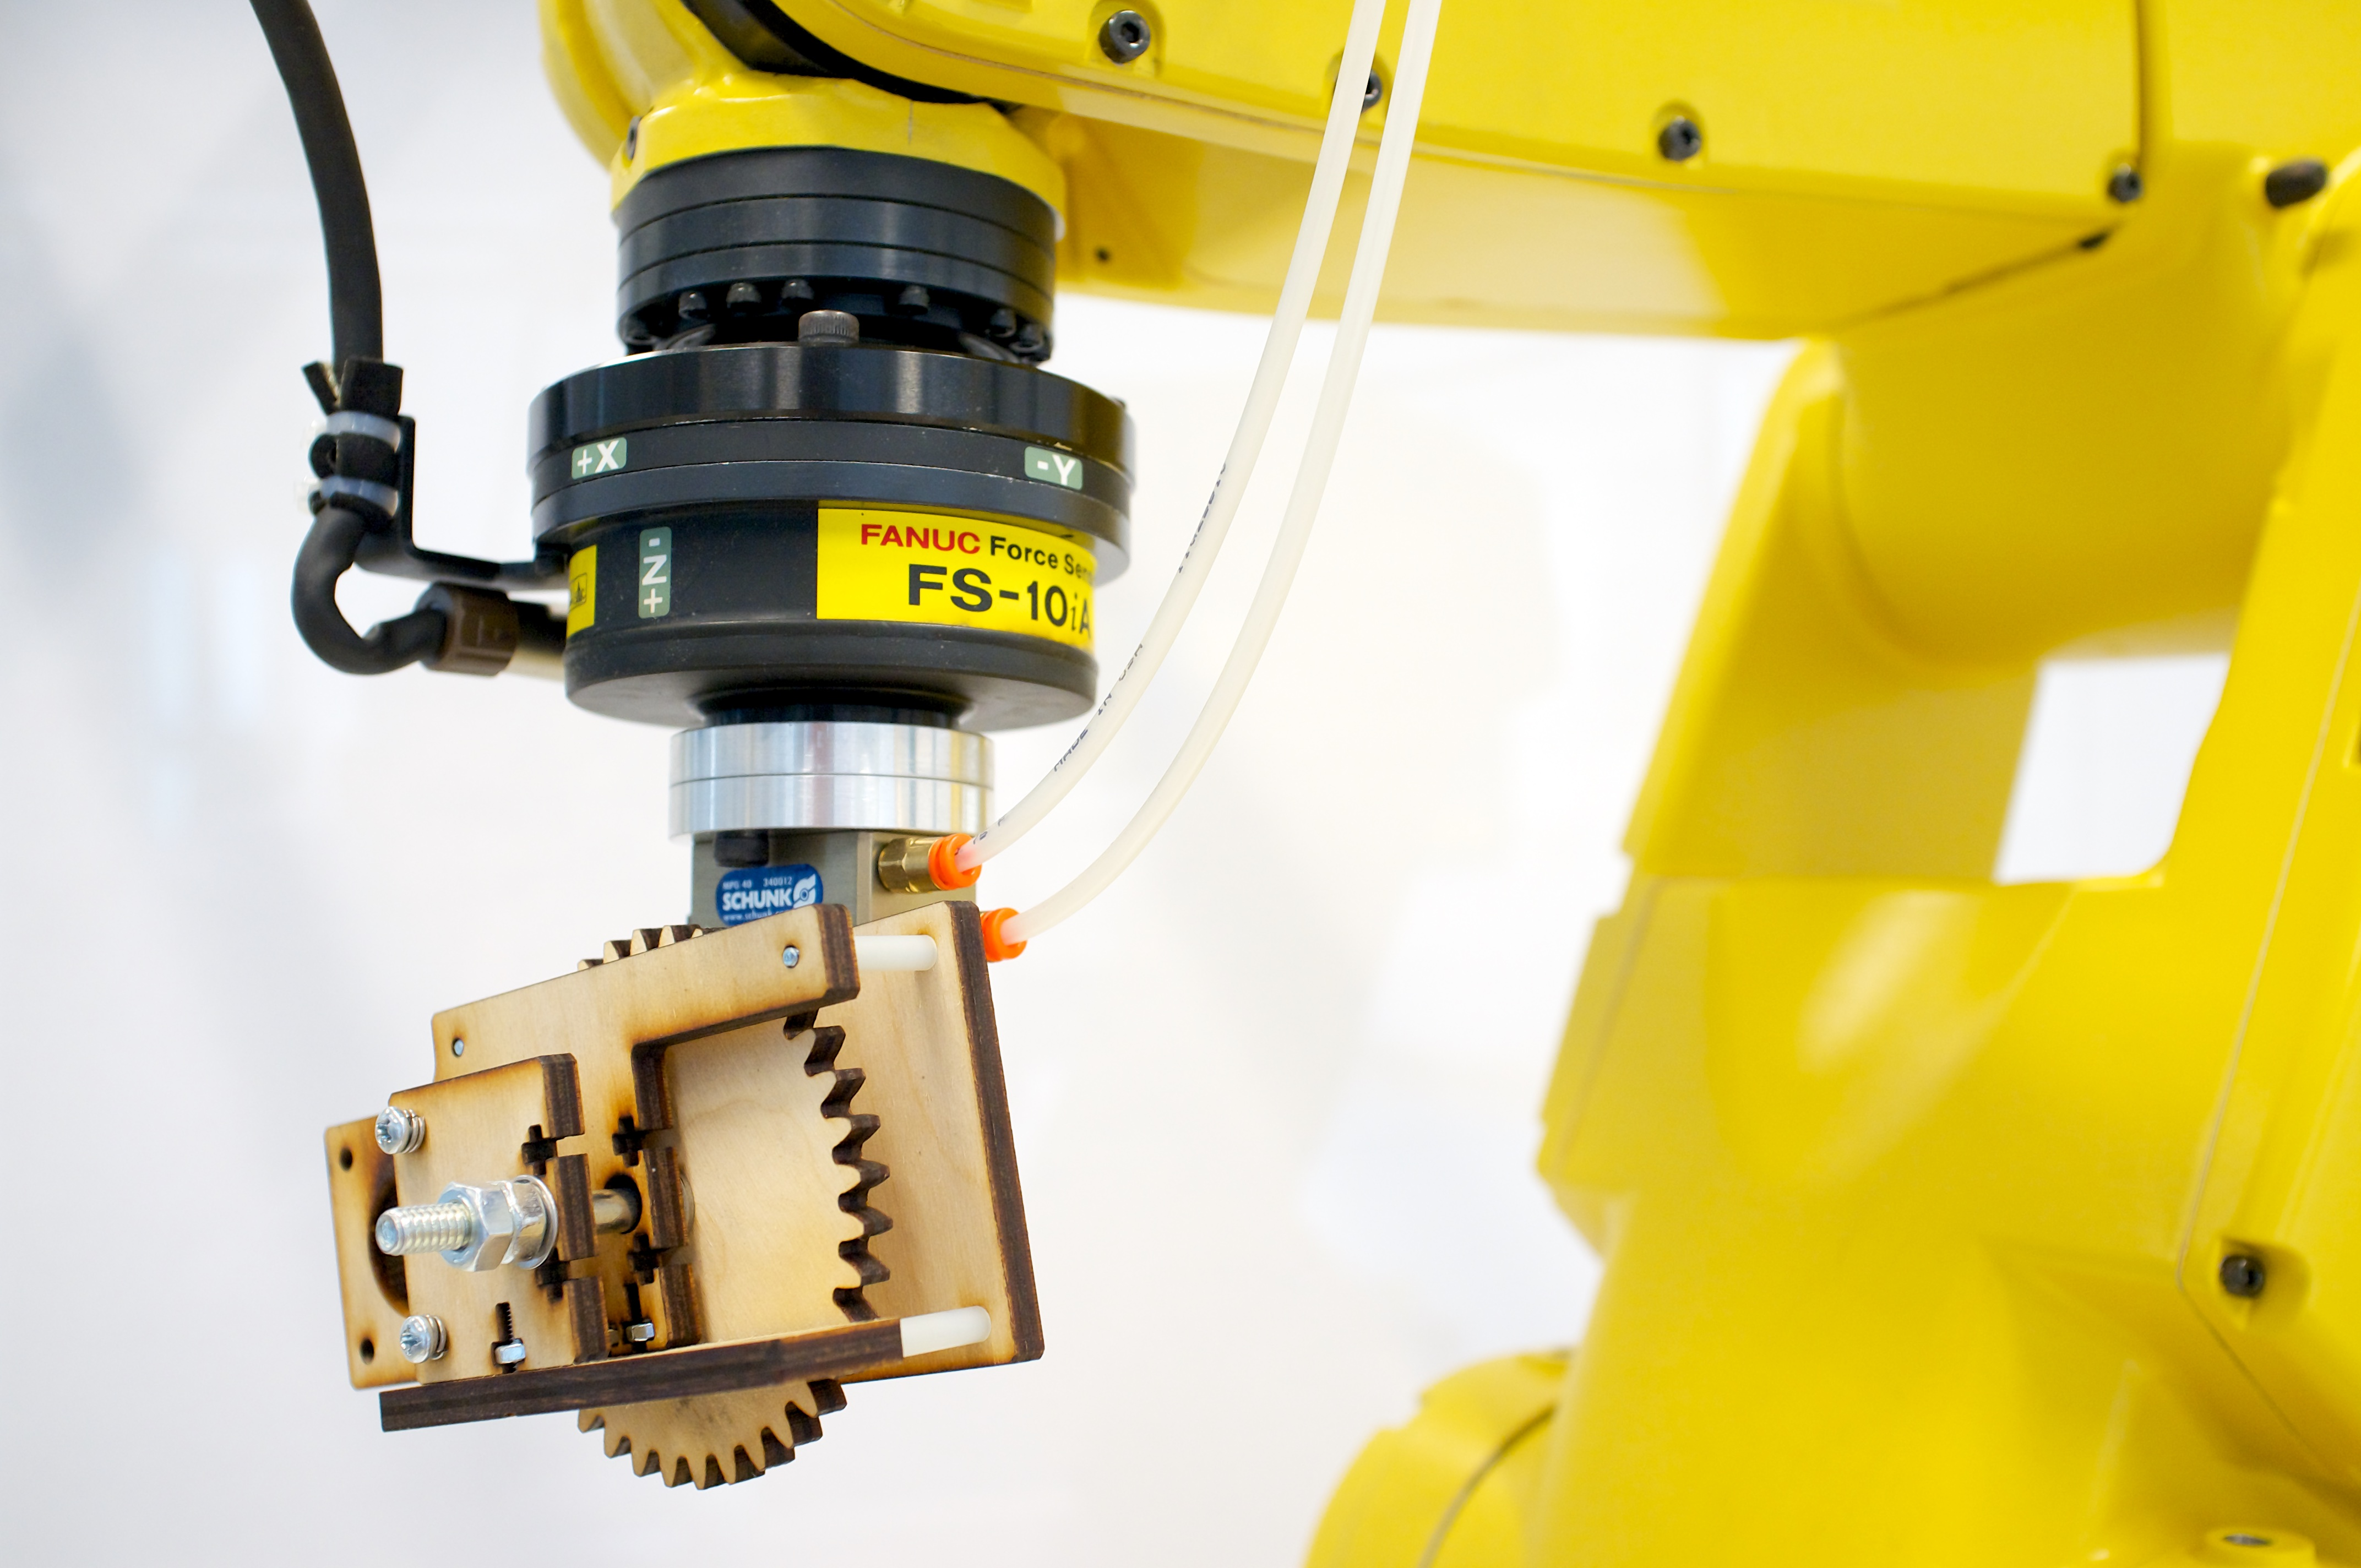
\includegraphics[width=0.5\textwidth]{./figures/extruder-prototype-2}
\caption{A photograph of the mounted prototype.}
\label{fig:prototype extruder}
\end{figure}

Figure~\ref{fig:extruder iso} presents a rendering of the final extruder design (manufacturing drawings will be created over winter break and the extruder will be machined immediately at the beginning of next semester). Figure~\ref{fig:extruder drawing} provides general dimensions and annotations to fully present the extruder design concept. The final design is significantly smaller than the initial design, will require less machining, and uses less fastening hardware. The size decrease was accomplished by using smaller gears (50\% scaled versions of gears dimensions taken from \emph{SDP-SI}\footnote{\url{http://www.sdp-si.com/}} and located the stepper motor directly beneath the FANUC grippers. As part of the design process the gears were laser-cut, and physically tested to ensure that the teeth would not shear off under a load less than the stall torque of the stepper motor, before being fully committed to this design. The stepper motor (Sparkfun ROB - 10846) outputs 68 oz.in of torque and has a resolution of 400 steps/revolution. Two laser-cut 1/4 inches thick acrylic gears step up the torque to 204 oz.in.\footnote{Most extruders in the 3D printing community use analogous stepper motors and utilize gear trains to step up the torque. Common gear ratios range from 2:1 to 4:1 depending on the specific qualities of the filament. Given that the specifics of our filament are not yet fully determined, the mean value was used.} A partially threaded 1/4-20 screw will be notched on the mill to contain teeth-like features along a portion of its length. At a depth of 1/2 mm, these teeth will grip the filament and push it into the extruder. The screw rides along two bronze PTFE-coated bearings to ensure smooth rotation during printing. Two adjustment plates locate a bearing just opposite the screw to provide counter-pressure during printing. The plates are secured in place using four screws, which can be loosened or tightened to adjust the distance between the screw and bearing to accommodate different filament sizes. Shims or spring washers may have to be utilized to located this adjustable mechanism in its optimal position for the official CFRP.\\

The extruder will be machined with aluminum to provide rigidity. Many 3D printers utilize 3D printed bodies for mounting RepRap hardware but the associated poor tolerances and material flexibility are not ideal for the Curved Layer Carbon Fiber 3D printer. Machining our own extruder out of aluminum will allow us to easily implement any future adjustments if the need arises, ensures all mechanisms will align properly, keeps the structure from deflecting under the dynamic loads of large arm movements, and could withstand an impact to the FANUC cage with minimal or no damage. The entire extruder assembly secures to the FANUC gripper with four metric screws in such a way to provide moment resistance about all three rotational degrees of freedom.\\

\begin{figure}[h!]
\centering
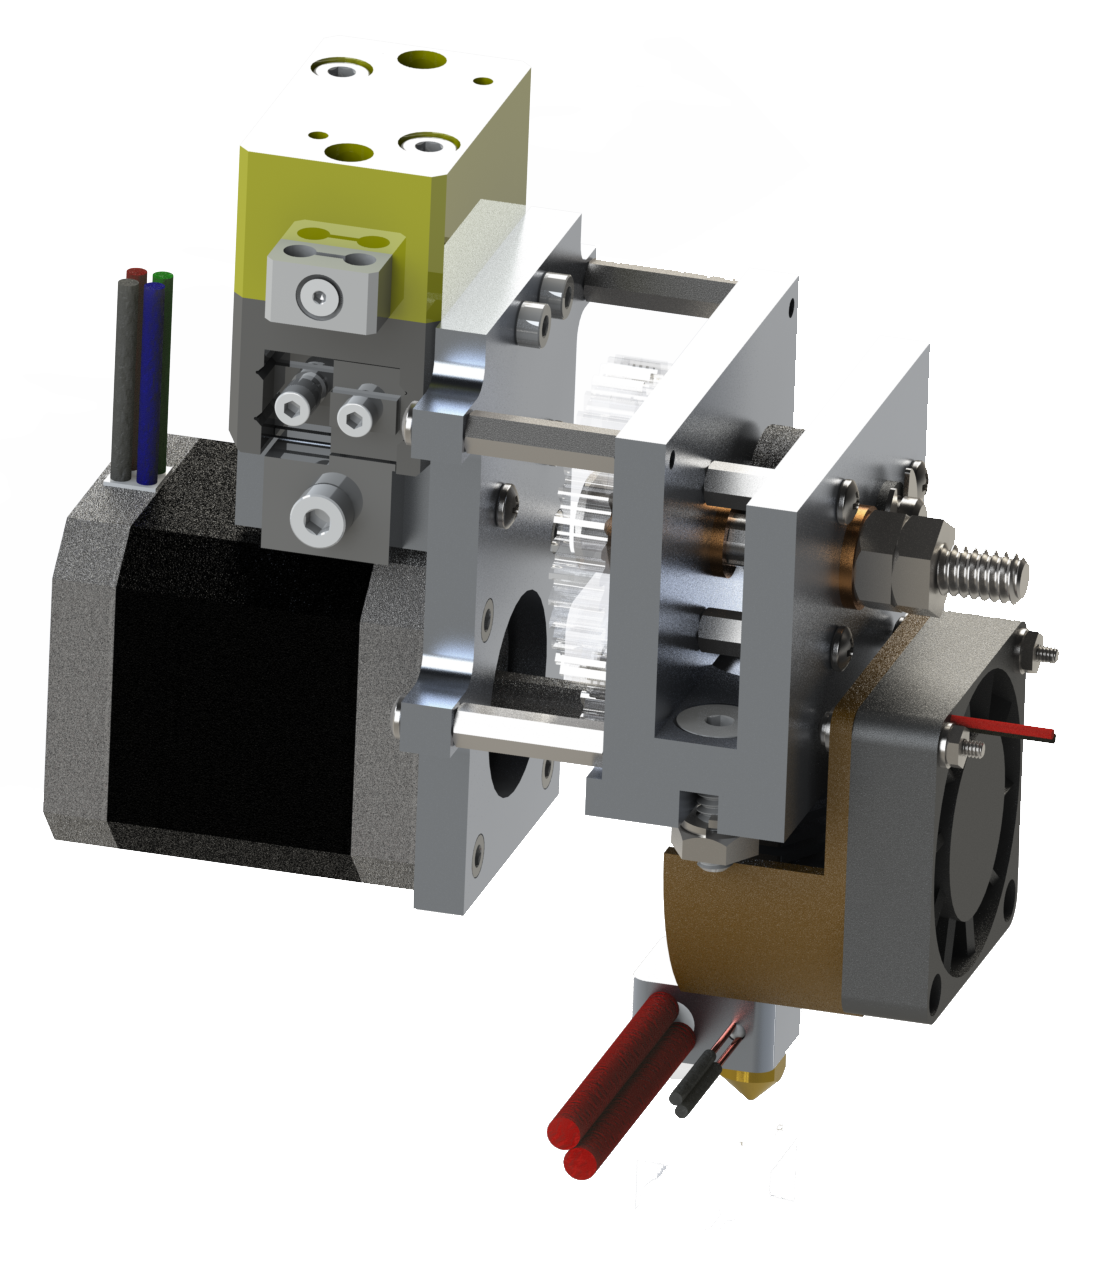
\includegraphics[width=0.5\textwidth]{./figures/extruder-iso}
\caption{An isometric render of the final extruder design.}
\label{fig:extruder iso}
\end{figure}

%\begin{figure}[htp]
%\centering
%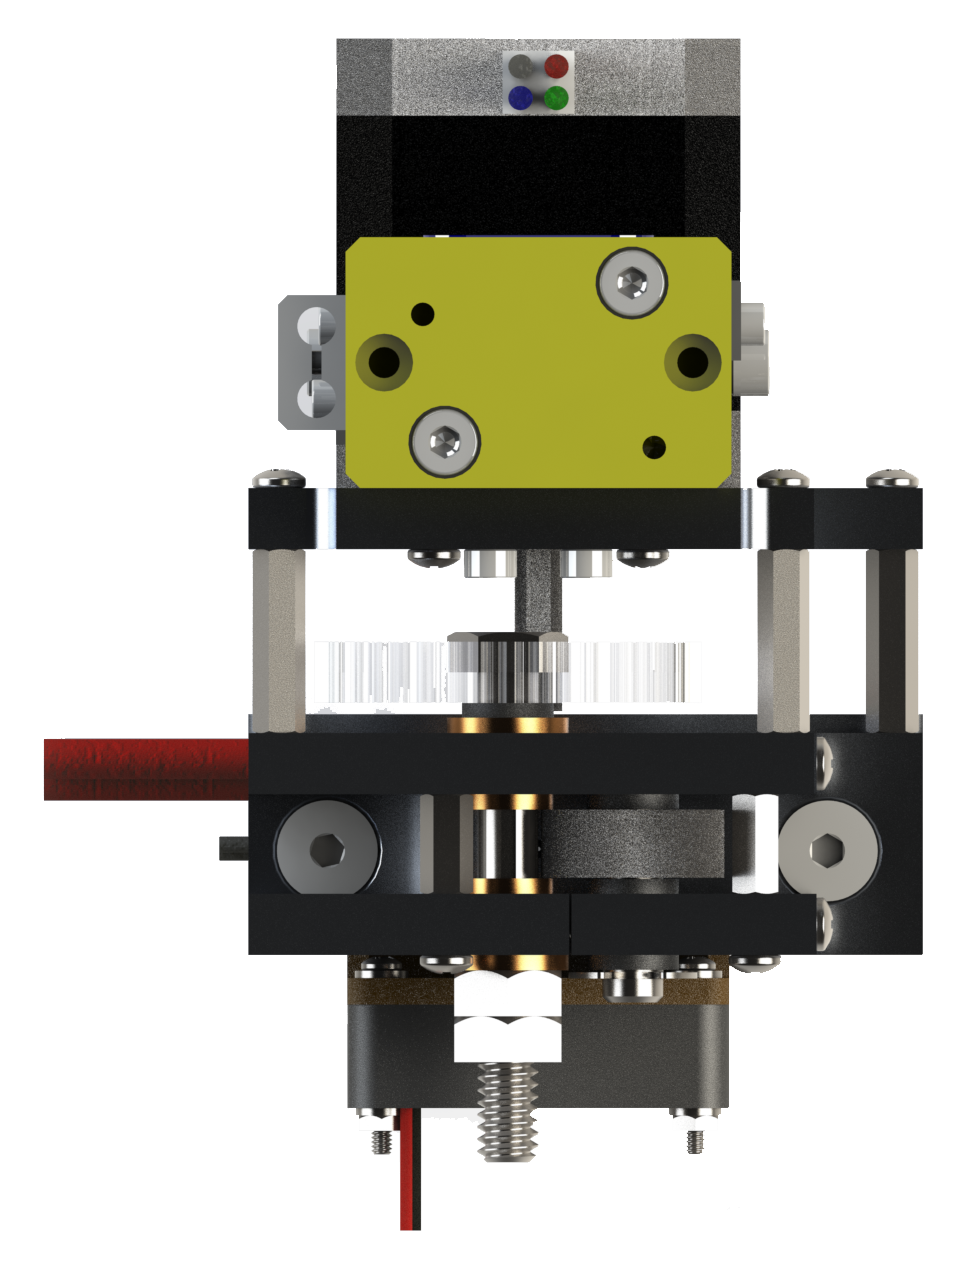
\includegraphics[width=0.25\textwidth]{./figures/extruder-top}
%\caption{A top view render of the final extruder design.}
%\label{fig:extruder top}
%\end{figure}

%\begin{figure}[htp]
%\centering
%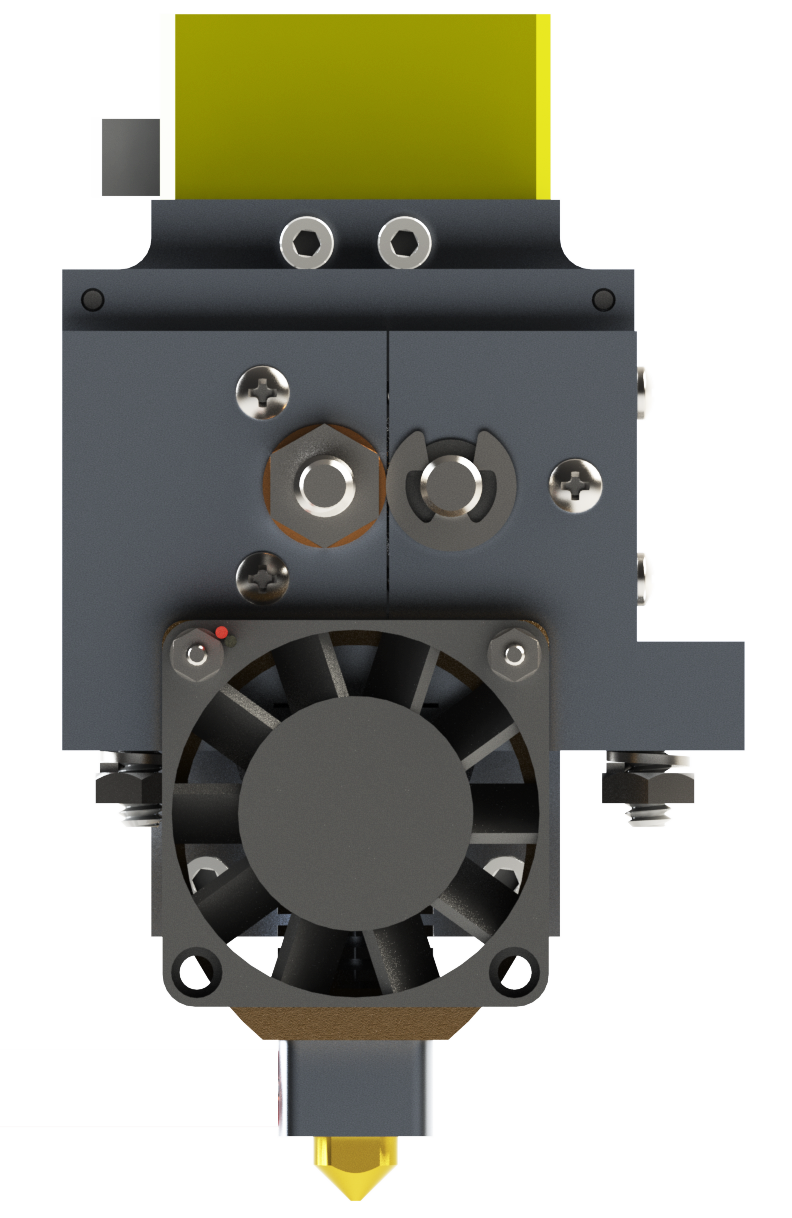
\includegraphics[width=0.25\textwidth]{./figures/extruder-front}
%\caption{A front view render of the final extruder design.}
%\label{fig:extruder front}
%\end{figure}

\begin{figure}[h!]
\centering
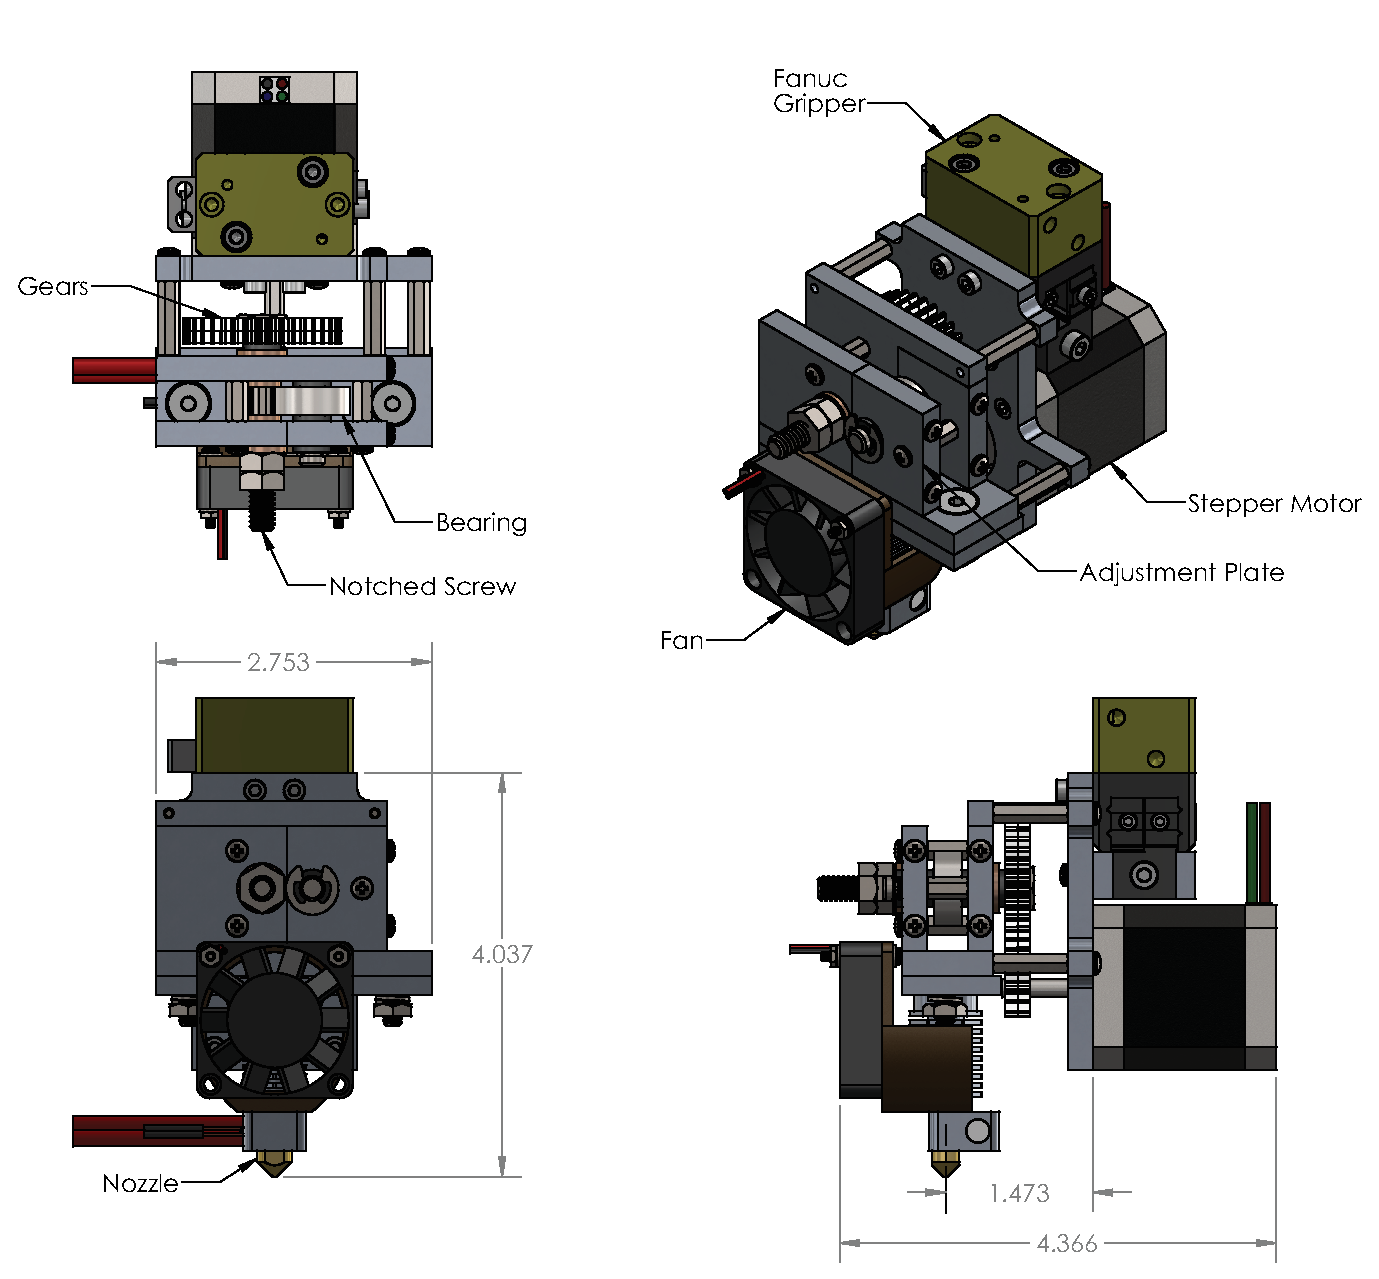
\includegraphics[width=1\textwidth]{./figures/extruder-drawing}
\caption{A general drawing of the final extruder design.}
\label{fig:extruder drawing}
\end{figure}

\clearpage

\subsection{Control Electronics}
\indent 

The extruder is controlled by a Megatronics control board, which was developed for the RepRap open source 3D printer project. The board contains all the necessary electronics to drive a Cartesian coordinate based FDM desktop 3D printer. The board can drive numerous positioning and extruder motors, heating elements, sensors, displays, and more. Because the FANUC robot handles the extruder positioning, the Megatronics board will be used to control the extruder elements only. 

When used in RepRap printers, the Megatronics board is typically used with one of several open source firmwares that are also associated with the RepRap project. Because these firmwares were designed with Cartesian desktop FDM printers in mind, they work well with the Megatronics board. The chosen firmware is uploaded to the board using a USB cable. For the FANUC-mounted extruder, a suitable firmware will be chosen and modified to work with the FANUC robot.

The firmware will be modified to control only the components present on the FANUC-mounted extruder. The firmware's timing functions must be modified as well. Normally, the firmware calculates its own filament feed rates and motor speeds. Because the FANUC controller is much less flexible than the RepRap firmware, the firmware will be modified to monitor the FANUC robot speed and position, and act accordingly. 

\subsection{Slicing Algorithm and Layer Generation}

\indent

sample text
